\chapter{The Menthal Story [SP]}
\label{chap:menthal_story}
Such devices as smartphones became an integral part of modern life.
People use them not only for communication, but for a plenty of other purposes, like reading books, surfing in the Internet, playing games, etc.
However, most of the users cannot correctly estimate the time spent on their phone during the day.
Besides, information about how people use their phones can be analysed from different sides.
Psychological research, statistical calculations, medicine and healthcare projects, advertising, - these are several examples of where such data can yield a profit.
Menthal is an application that is designed specifically for these purposes.
This chapter describes the main functionality and technical details of this application.

Nowadays mobile/smartphone excessive usage becomes a critical problem.
People constantly use these devices, making calls, sending messages, surfing in the Internet or just playing.
People are distracted by their phones even on personal meetings, parties and dates.
When a person leaves his phone at home, quite often he feels nervous and irritated.
Some people suffer from a cellphone vibration syndrome, when one feels as if a cellphone is vibrating but in fact it is not.
Sometimes they unlock the phone and check messages or social network pages unconsciously, just to make sure that nothing new has happened. 

The crucial problem is that people are not able to detect that they concentrate on their smartphones too much.
Few of them can correctly estimate the daily usage period of the device.
First, it is difficult to evaluate yourself, take a detached view on your behavior.
For example, one can unlock his phone 45 times per day and use it for 2 minutes on average.
However, in the end of the day it sums up to 1,5 hours.
This fact can surprise the user, because his estimated frequency of interaction with a phone and usage time would be much smaller.
Second, even if a person can correctly assess the wasted time, it is morally unpleasant to confirm these figures.
For instance, one plays a game on his smartphone instead of working on important task that has to be accomplished.
Finally, the task is not finished, the person realizes that the reason was that mobile game, but it is easier to say that there was not enough time to complete the task.  
Thus, exterior assessment mechanism is needed to calculate how much time a user spend on his smartphone, what applications he uses and when.    

At the same time, there is no proper study how people use their phones.
Currently most of the researches in the field of human-smartphone interaction involve direct interaction with a user group, by means of questionnaires and interviews.
Recently special software applications for smartphones to keep track of user actions emerge.
However, they still require the interaction with users, showing dialogue boxes and asking questions.
It introduces a certain bias into the results of the research, because a user gets distracted by this interference.
Only an application that is invisible for users can help to make a complete and thorough research.

The results of human-smartphone study can be used in various fields.
For example, France introduces a rule to switch off work phones after 18:00 and till 9:00, to protect employees from official duties outside office hours.
To perform such introduction, it is important to investigate how people of various professions use their work phone.
This research can help to detect the cases when it is actually necessary to block the phones.
In some cases maybe it is sufficient to block only particular functions, such as emails or text messages.

Moreover, it is essential to determine how people use their smartphones to make user-friendly application interfaces. 
An application interface has a big influence on user.
Developers can make it attractive and handy, that encourages users to use the application again even if there is no actual necessity.
If a person wants to decrease the time spent on the smartphone, a special enhanced interface can help.
For example, the phone can warn user when he spends too much time using the device during the day.  

As a result, there are two problems that have to be solved. 
On the one hand, there is a need to provide a user with his smartphone use information.
On the other hand, it is necessary to supply researches with a tool that tracks smartphone usage.
Menthal, an application for smartphones, combines these two features and provides solutions for both of these problems. 

\section{Study}
Menthal is an application that gathers phone usage data and stores it on a server for further analysis, providing user with a feedback.
Phone usage data includes the number of times user unlocks his phone, the number of performed calls and sent SMS, etc.
The user receives a feedback about the smartphone usage statistics that is provided by the server.
In this case Menthal uses the same concept as Google: it grants users a free service in return to data.
This approach works well, and the high number of Menthal users demonstrates it. 

Prior to present Menthal application a pilot study was conducted. 
It was a psychological experiment on 49 participants.
During 5 weeks their telephone/SMS usage was measured by means of a mobile phone application.
The personality dimensions were determined using questionnaire.
The goal of this study was to detect a connection between smartphone usage patterns and personality traits.

In contrast to other similar attempts, this work uses automatized approach for gathering information instead of self-report data.
The application tracks tuples for calls of the format (anonymized number, start time, end time, in/out).
SMS tuples have a form (anonymized number, length of the message, time sent for outgoing messages / time received, time read for incoming SMS).
The application is not visible for the user, uploading data to the server automatically.
Later collected data is analysed on the server in the context of personality traits.
Among the result of the study one can observe a positive correlation between extraversion and the number and frequency of telephone calls.

\section{Technical Details}
This experiment develops into an independent smartphone application for mass usage. 
It collects data, providing user with a feedback and supplying psychologists with information that can be analysed later on.
Figure~\ref{fig:menthal_architecture} illustrates the Menthal architecture.
The application includes a client and a server part, that interact with each other via HTTPS.

\begin{figure}[h]
  \centering
  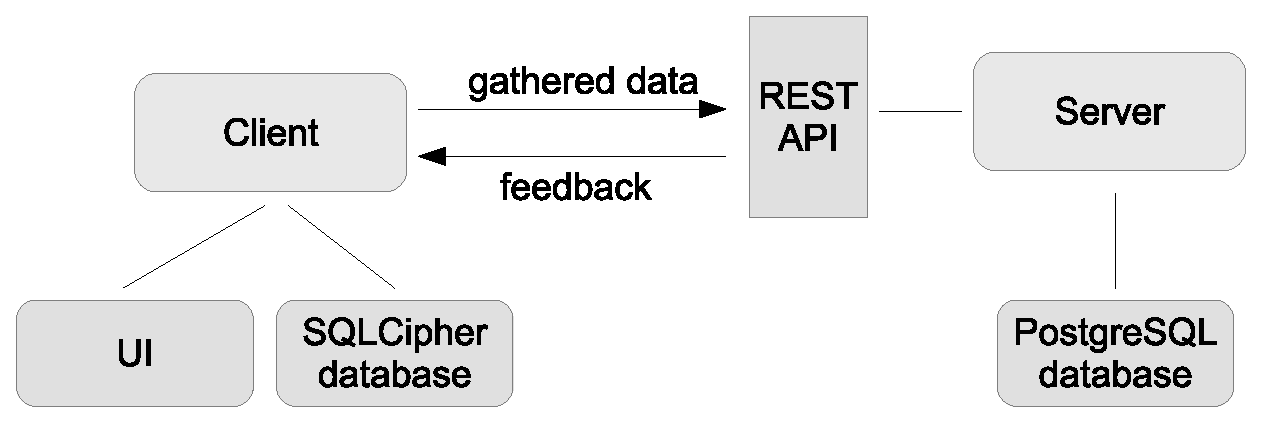
\includegraphics [width=0.7\textwidth]{images/Menthal_architecture}
  \caption{Menthal architecture}
  \label{fig:menthal_architecture}
\end{figure}

The client part consists of an Android application installed on a smartphone.
It keeps track of all the user activity during the day.
All the activities are stored as \textit{events}.
Each event contains such data as id, event type, timestamp, data itself and some additional information.
The main types of events are: SMS\_RECEIVED, SMS\_SENT, CALL\_RECEIVED, CALL\_OUTGOING, CALL\_MISSED, SCREEN\_UNLOCK, \\*
 SCREEN\_LOCK, LOCALISATION.
The information gathering process is hidden from users, the application runs in the background, automatically sending data to the server.

The application gathers this data from different sources, using standard Android operating system API.
For example, to get the information about phone lock/unlock, it listens to the corresponding events and handles them.
To be aware of application usage, Menthal periodically (every 2 seconds) checks the current top application in the application stack of the smartphone.
If the application detects that the application has been changed, it writes the event into the database, adding a timestamp.
Catching a lock event is also used as a sign that the current application was changed and leads to a new record into the database.
The information about phone calls and sms can be queried from a local smartphone storage.
Every six hours Menthal checks whether the day is changed and if it does, it makes a new query to the local storage to get the latest information about performed calls and sent/received sms. 
 
\mnote{Menthal GUI}
Menthal has a user interface to provide users with a feedback. 
The main screen shows a 'score' - the relative phone usage measurement.
Using this value, one could check how intensively he uses his phone today comparing to previous days statistics.
UI provides also additional functionality.
It shows overall daily/weekly/monthly statistics about the phone usage such as most used application, number of calls or the number of times user unlocked the phone.
After a short questionary it can display personality characteristics diagram, that includes five sides: extraversion, neuroticism, openness, conscientiousness, agreeableness.
Furthermore a user can check the list of contacts with whom he communicates more often over a period of time.
The next screen shows the daily time spenditure with the phone for the last 30 days.
The application is able to keep track of user mood, periodically checking his current state of mind.
Using smartphone's GPS receiver, Menthal can determine and show on map the user location.
Moreover the application gives an opportunity to put a time limit on a particular application, so when the limit is exceeded the phone warns a user about that.

\begin{figure}[h]
\centering
\begin{minipage}{.5\textwidth}
  \centering
  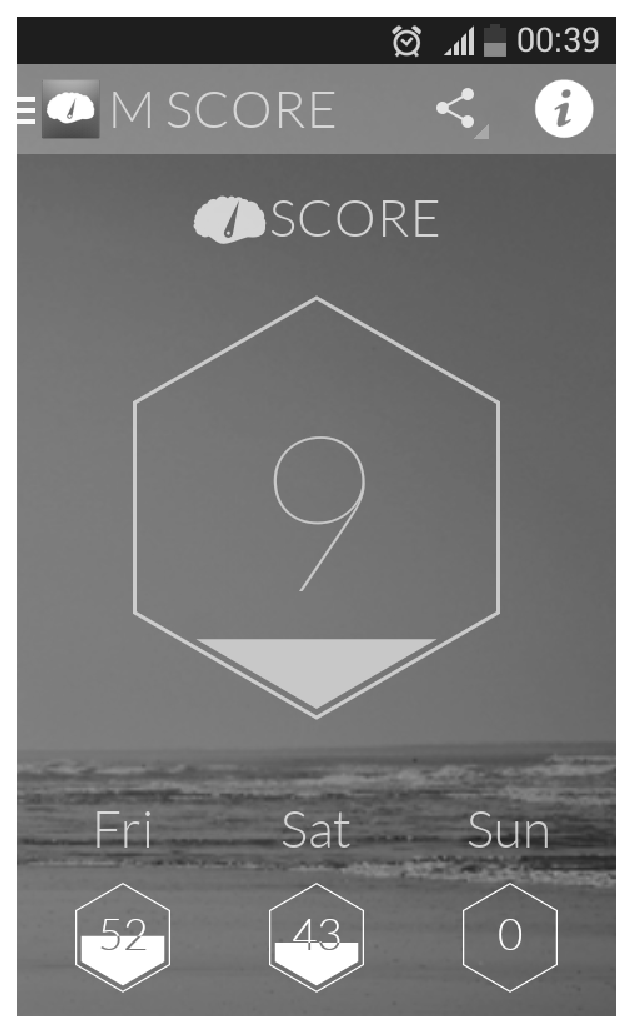
\includegraphics [width=.8\textwidth]{images/Menthal_GUI_mainscreen}
  \caption{Start screen}
  \label{fig:menthal_gui_mainscreen}
\end{minipage}%
\begin{minipage}{.5\textwidth}
  \centering
  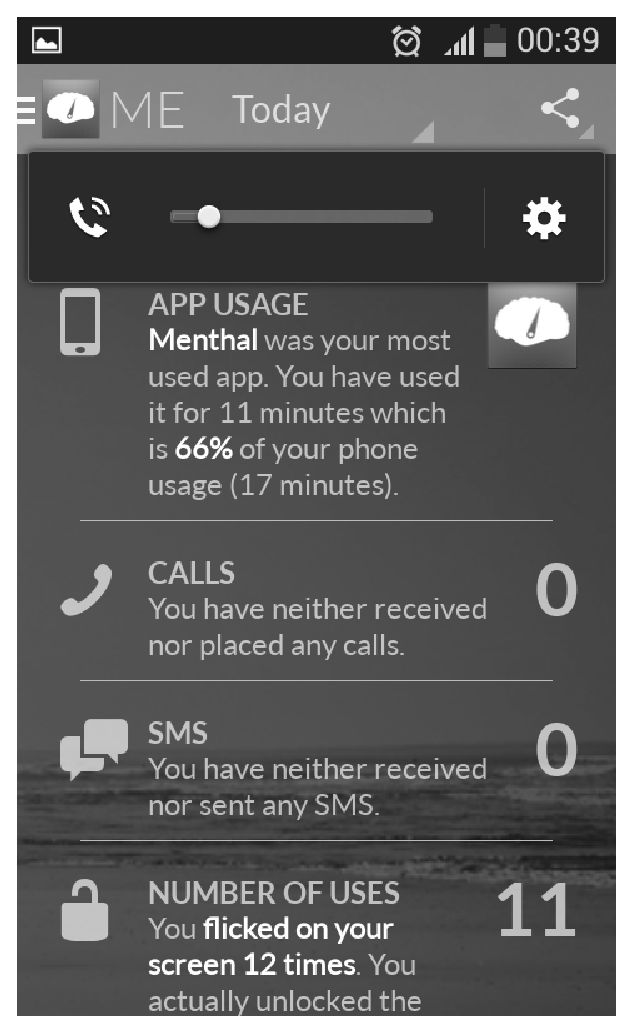
\includegraphics [width=.8\textwidth]{images/Menthal_GUI_me}
  \caption{Personal statistics}
  \label{fig:menthal_gui_me}
\end{minipage}
\end{figure}

\begin{figure}[h]
\centering
\begin{minipage}{.5\textwidth}
  \centering
  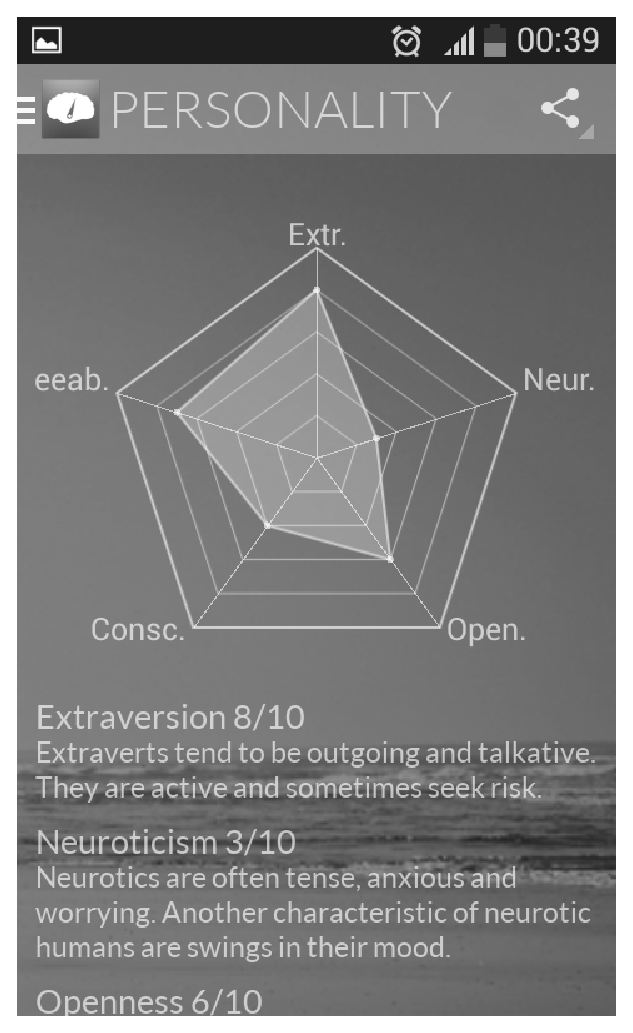
\includegraphics [width=.8\textwidth]{images/Menthal_GUI_personality}
  \caption{Personality characteristics}
  \label{fig:menthal_gui_personality}
\end{minipage}%
\begin{minipage}{.5\textwidth}
  \centering
  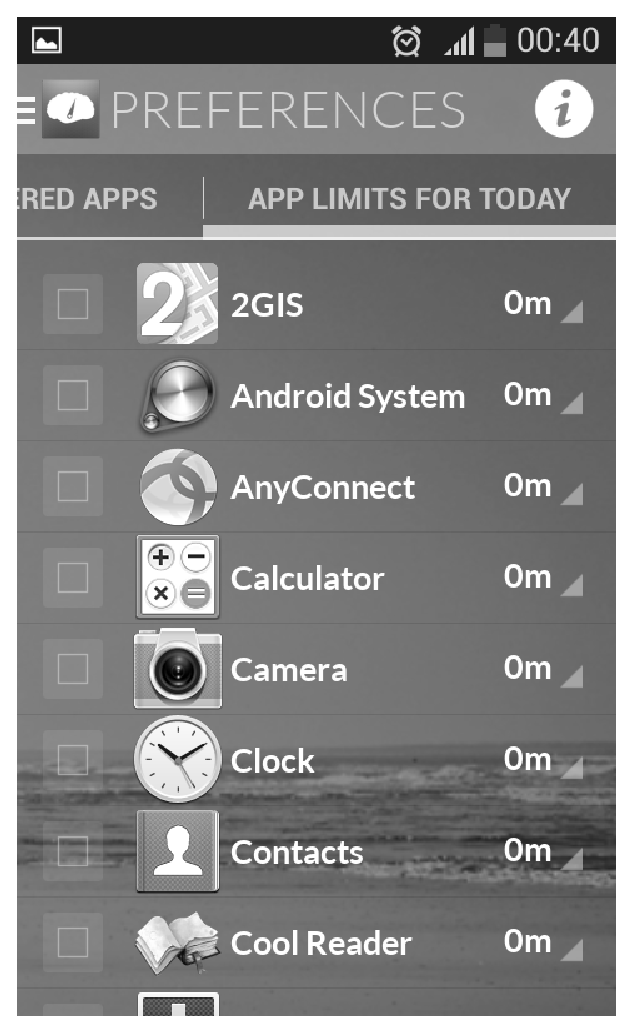
\includegraphics [width=.8\textwidth]{images/Menthal_GUI_preferences}
  \caption{Time limits preferences}
  \label{fig:menthal_gui_preferences}
\end{minipage}
\end{figure}

All the gathered data is temporarely stored on a phone in a cryptographically protected SQLCipher database.
Every time a new event is created, the application increases a special counter by 1.
When this value reaches 50, Menthal performs the following steps:

1) Obtain all the data from the SQLCipher database.

2) Convert it into JSON.

3) Send it to the server.

4) Wait for the reply.

5) If the server does not respose, try again in approximally 2 minutes. 

6) If the acknowledgment is received, delete the data that was sent from the SQLCipher database.

However, this is done only when a phone is connected to WiFi to avoid unnecessary charges for the user.
If the phone was not connected to WiFi during the day, Menthal still needs to send the data.
In this case the application sends it at random time between 1:00 - 6:00 at night via 3G.
All the data is sent in batches, where one batch contains no more than 50 events.

\mnote{information security}
Menthal uses secure connection, encryption of sensitive data and authentication mechanism to guarantee information security.
Communication between the client and the server goes through HTTPS.
This protocol is designed to provide a secure communication over a computer network. 
OAuth 1.0a protocol guarantees an authorization control.
When a client connects to the server the very first time, it receives a token.
Later the client sends this token with every message and the server uses it for authentication.
On the phone the data is stored in SQLCipher database.
This database uses 256 bit AES encryption for storing information in a secure way.
Moreover, Menthal hashes the sensitive data, such as the contact names or the phone numbers via SHA2. 

On the Server side Menthal has a cluster of 3 machines.
A PostgreSQL database is replicated between two of them.
One of these machines serves as a master node and another as a slave node.
The third machine hosts a key-value store that works as a read cache, message and task queues and a web application.
 
Menthal recently gained popularity among users.
It happened when the application was covered in mass media.
The articles in newspapers and interview with a project leader lead to the explosive increase of the number of users.
Almost 50 000 persons have this application installed on their phones.
All of these devices periodically send collected information to the server, that sums up to a vast amount of data.
Totally around 34Gb of information is received per day, that is almost 1Tb per month.
All these factors have a significant influence on the application performance.
The Menthal server side becomes overflowed and is not able to write all incoming data into the database, not to mention providing a feedback.
Therefore, the application requires a new, enhanced server-side architecture that can meet the new requirements.